\documentclass{article}
\usepackage{booktabs,geometry,graphicx,amsmath}
\geometry{margin=1in}
\title{A side check: MMD-LOCO against vanilla MMD\\on a covariate shift}
\author{}
\date{}
\begin{document}
\maketitle

This note is not the FSDS horse-race. It only asks whether the leave-one-coordinate
MMD scores, turned into a single permutation statistic, detect a mean shift in $X$
more often than the joint MMD on the same kernel.

The kernel is $\exp(-\gamma\|x-y\|^2)$ with $\gamma$ equal to one over the median
pooled squared distance. $\gamma$ is computed once on the observed pool and held
fixed. Dropping coordinate $j$ subtracts that coordinate's squared differences from
the three distance matrices, which is the joint kernel on the remaining coordinates
at the same $\gamma$. The vector of interest is $\mathrm{MMD}^2-\mathrm{MMD}^2_{-j}$.
Two scalars are tested: the maximum coordinate, and the sum of the positive coordinates.
The baseline is the unbiased $\mathrm{MMD}^2$ itself. A normalized version,
$\mathrm{NAMMD}^2=\mathrm{MMD}^2_u/\sqrt{\bar k_{xx}\bar k_{yy}}$, is carried along
because the same drop applies to it. Each test uses the same label permutations.
The $p$-value is $(1+\#\{T_b\ge T\}) / (B+1)$.

Each batch has $n=120$ reference rows and $n$ new rows. Coordinates are standard
normal, independent in the main grid, with an AR(1) check beside it. The new batch
adds a constant to the first $s$ coordinates. $B=199$ permutations and
$80$ Monte Carlo replicates. The dashed line in the figure is $\alpha=0.05$.
ECMMD is omitted: it needs a response and is a conditional discrepancy, not a test of $P(X)$.

On one shifted coordinate the maximum is the more sensitive of the two.
At $p=50$ and shift $0.60$, max LOCO rejects in $0.95$ of the $80$ replicates
and vanilla MMD in $0.65$; $25$ replicates are rejected only by the maximum
and $1$ only by MMD. At $p=20$ and shift $0.50$ the rates are $0.85$ and $0.60$
($22$ only by the maximum, $2$ only by MMD).
A shift in every coordinate reverses this. At $p=50$ and shift $0.10$,
vanilla MMD rejects in $0.81$ and the maximum in $0.19$
($50$ replicates only by MMD). The sum of the positive coordinates stays nearer
the joint statistic on that dense shift ($0.65$) than the maximum does.
Null rejection across the grid sits between $0$ and $0.11$.

\begin{table}[p]
\centering
\caption{Independent coordinates. Rejection rate at $\alpha=0.05$. Each row is one covariate-shift cell. The six statistics share the kernel, the bandwidth, and the permutations.}
\resizebox{\textwidth}{!}{%
\begin{tabular}{llcccccc}
\toprule
$p$ & $s$, shift & MMD & max LOCO & positive-sum LOCO & NAMMD & max NAMMD-LOCO & positive-sum NAMMD-LOCO \\
\midrule
20 & 1, 0.00 & 0.04 & 0.07 & 0.07 & 0.04 & 0.06 & 0.06 \\
20 & 1, 0.20 & 0.16 & 0.12 & 0.23 & 0.16 & 0.14 & 0.20 \\
20 & 1, 0.35 & 0.33 & 0.46 & 0.33 & 0.33 & 0.44 & 0.31 \\
20 & 1, 0.50 & 0.60 & 0.85 & 0.72 & 0.60 & 0.84 & 0.68 \\
20 & 1, 0.80 & 0.99 & 1.00 & 0.99 & 0.99 & 1.00 & 0.99 \\
20 & 4, 0.00 & 0.05 & 0.11 & 0.10 & 0.05 & 0.10 & 0.05 \\
20 & 4, 0.20 & 0.39 & 0.21 & 0.34 & 0.39 & 0.24 & 0.35 \\
20 & 4, 0.35 & 0.93 & 0.80 & 0.89 & 0.93 & 0.84 & 0.93 \\
20 & 4, 0.50 & 1.00 & 0.97 & 1.00 & 1.00 & 0.99 & 1.00 \\
20 & 4, 0.75 & 1.00 & 1.00 & 1.00 & 1.00 & 1.00 & 1.00 \\
20 & 20, 0.00 & 0.05 & 0.03 & 0.05 & 0.05 & 0.03 & 0.06 \\
20 & 20, 0.10 & 0.38 & 0.12 & 0.29 & 0.38 & 0.14 & 0.35 \\
20 & 20, 0.20 & 1.00 & 0.49 & 1.00 & 1.00 & 0.72 & 1.00 \\
20 & 20, 0.35 & 1.00 & 0.95 & 1.00 & 1.00 & 1.00 & 1.00 \\
20 & 20, 0.50 & 1.00 & 0.99 & 1.00 & 1.00 & 1.00 & 1.00 \\
50 & 1, 0.00 & 0.06 & 0.03 & 0.06 & 0.06 & 0.03 & 0.09 \\
50 & 1, 0.40 & 0.30 & 0.54 & 0.36 & 0.30 & 0.54 & 0.30 \\
50 & 1, 0.60 & 0.65 & 0.95 & 0.80 & 0.65 & 0.95 & 0.74 \\
50 & 1, 0.85 & 0.94 & 1.00 & 0.97 & 0.94 & 1.00 & 0.94 \\
50 & 1, 1.15 & 1.00 & 1.00 & 1.00 & 1.00 & 1.00 & 1.00 \\
50 & 4, 0.00 & 0.04 & 0.00 & 0.04 & 0.04 & 0.00 & 0.04 \\
50 & 4, 0.30 & 0.57 & 0.49 & 0.59 & 0.57 & 0.53 & 0.61 \\
50 & 4, 0.50 & 0.99 & 0.99 & 1.00 & 0.99 & 1.00 & 1.00 \\
50 & 4, 0.75 & 1.00 & 1.00 & 1.00 & 1.00 & 1.00 & 1.00 \\
50 & 4, 1.00 & 1.00 & 1.00 & 1.00 & 1.00 & 1.00 & 1.00 \\
50 & 50, 0.00 & 0.04 & 0.05 & 0.06 & 0.04 & 0.05 & 0.05 \\
50 & 50, 0.10 & 0.81 & 0.19 & 0.65 & 0.81 & 0.24 & 0.76 \\
50 & 50, 0.18 & 1.00 & 0.54 & 1.00 & 1.00 & 0.74 & 1.00 \\
50 & 50, 0.30 & 1.00 & 0.85 & 1.00 & 1.00 & 1.00 & 1.00 \\
50 & 50, 0.45 & 1.00 & 1.00 & 1.00 & 1.00 & 1.00 & 1.00 \\
\bottomrule
\end{tabular}}
\end{table}
\clearpage
\begin{table}[p]
\centering
\caption{AR(1) correlation 0.5. Rejection rate at $\alpha=0.05$. Each row is one covariate-shift cell. The six statistics share the kernel, the bandwidth, and the permutations.}
\resizebox{\textwidth}{!}{%
\begin{tabular}{llcccccc}
\toprule
$p$ & $s$, shift & MMD & max LOCO & positive-sum LOCO & NAMMD & max NAMMD-LOCO & positive-sum NAMMD-LOCO \\
\midrule
20 & 1, 0.00 & 0.05 & 0.03 & 0.03 & 0.05 & 0.03 & 0.05 \\
20 & 1, 0.35 & 0.25 & 0.44 & 0.29 & 0.25 & 0.44 & 0.26 \\
20 & 1, 0.60 & 0.61 & 0.97 & 0.78 & 0.61 & 0.96 & 0.75 \\
20 & 20, 0.00 & 0.05 & 0.03 & 0.04 & 0.05 & 0.03 & 0.06 \\
20 & 20, 0.20 & 0.91 & 0.42 & 0.69 & 0.91 & 0.56 & 0.84 \\
20 & 20, 0.40 & 1.00 & 0.86 & 0.99 & 1.00 & 1.00 & 1.00 \\
\bottomrule
\end{tabular}}
\end{table}
\clearpage
\begin{table}[p]
\centering
\caption{Paired comparison with vanilla MMD on the same replicates. ``Only max'' counts replicates rejected by max LOCO and not by MMD. ``MMD, not max'' is the reverse. The last two columns are the same split for the sum of positive LOCO scores.}
\resizebox{\textwidth}{!}{%
\begin{tabular}{llccccccc}
\toprule
$p$ & $s$, shift & MMD & max LOCO & only max & MMD, not max & pos.\ sum & only pos.\ & MMD, not pos.\ \\
\midrule
20 & 1, 0.00 & 0.04 & 0.07 & 5 & 2 & 0.07 & 4 & 1 \\
20 & 1, 0.20 & 0.16 & 0.12 & 5 & 8 & 0.23 & 7 & 2 \\
20 & 1, 0.35 & 0.33 & 0.46 & 16 & 5 & 0.33 & 5 & 5 \\
20 & 1, 0.50 & 0.60 & 0.85 & 22 & 2 & 0.72 & 12 & 2 \\
20 & 1, 0.80 & 0.99 & 1.00 & 1 & 0 & 0.99 & 0 & 0 \\
20 & 4, 0.00 & 0.05 & 0.11 & 6 & 1 & 0.10 & 4 & 0 \\
20 & 4, 0.20 & 0.39 & 0.21 & 5 & 19 & 0.34 & 5 & 9 \\
20 & 4, 0.35 & 0.93 & 0.80 & 1 & 11 & 0.89 & 1 & 4 \\
20 & 4, 0.50 & 1.00 & 0.97 & 0 & 2 & 1.00 & 0 & 0 \\
20 & 4, 0.75 & 1.00 & 1.00 & 0 & 0 & 1.00 & 0 & 0 \\
20 & 20, 0.00 & 0.05 & 0.03 & 1 & 3 & 0.05 & 1 & 1 \\
20 & 20, 0.10 & 0.38 & 0.12 & 4 & 24 & 0.29 & 2 & 9 \\
20 & 20, 0.20 & 1.00 & 0.49 & 0 & 41 & 1.00 & 0 & 0 \\
20 & 20, 0.35 & 1.00 & 0.95 & 0 & 4 & 1.00 & 0 & 0 \\
20 & 20, 0.50 & 1.00 & 0.99 & 0 & 1 & 1.00 & 0 & 0 \\
50 & 1, 0.00 & 0.06 & 0.03 & 2 & 5 & 0.06 & 3 & 3 \\
50 & 1, 0.40 & 0.30 & 0.54 & 22 & 3 & 0.36 & 8 & 3 \\
50 & 1, 0.60 & 0.65 & 0.95 & 25 & 1 & 0.80 & 14 & 2 \\
50 & 1, 0.85 & 0.94 & 1.00 & 5 & 0 & 0.97 & 3 & 0 \\
50 & 1, 1.15 & 1.00 & 1.00 & 0 & 0 & 1.00 & 0 & 0 \\
50 & 4, 0.00 & 0.04 & 0.00 & 0 & 3 & 0.04 & 2 & 2 \\
50 & 4, 0.30 & 0.57 & 0.49 & 12 & 19 & 0.59 & 5 & 4 \\
50 & 4, 0.50 & 0.99 & 0.99 & 1 & 1 & 1.00 & 1 & 0 \\
50 & 4, 0.75 & 1.00 & 1.00 & 0 & 0 & 1.00 & 0 & 0 \\
50 & 4, 1.00 & 1.00 & 1.00 & 0 & 0 & 1.00 & 0 & 0 \\
50 & 50, 0.00 & 0.04 & 0.05 & 4 & 3 & 0.06 & 3 & 1 \\
50 & 50, 0.10 & 0.81 & 0.19 & 0 & 50 & 0.65 & 2 & 15 \\
50 & 50, 0.18 & 1.00 & 0.54 & 0 & 37 & 1.00 & 0 & 0 \\
50 & 50, 0.30 & 1.00 & 0.85 & 0 & 12 & 1.00 & 0 & 0 \\
50 & 50, 0.45 & 1.00 & 1.00 & 0 & 0 & 1.00 & 0 & 0 \\
20 & 1, 0.00, $\rho=0.5$ & 0.05 & 0.03 & 2 & 4 & 0.03 & 0 & 2 \\
20 & 1, 0.35, $\rho=0.5$ & 0.25 & 0.44 & 16 & 1 & 0.29 & 3 & 0 \\
20 & 1, 0.60, $\rho=0.5$ & 0.61 & 0.97 & 29 & 0 & 0.78 & 15 & 2 \\
20 & 20, 0.00, $\rho=0.5$ & 0.05 & 0.03 & 1 & 3 & 0.04 & 1 & 2 \\
20 & 20, 0.20, $\rho=0.5$ & 0.91 & 0.42 & 0 & 39 & 0.69 & 0 & 18 \\
20 & 20, 0.40, $\rho=0.5$ & 1.00 & 0.86 & 0 & 11 & 0.99 & 0 & 1 \\
\bottomrule
\end{tabular}}
\end{table}
\clearpage


\begin{figure}[p]
\centering
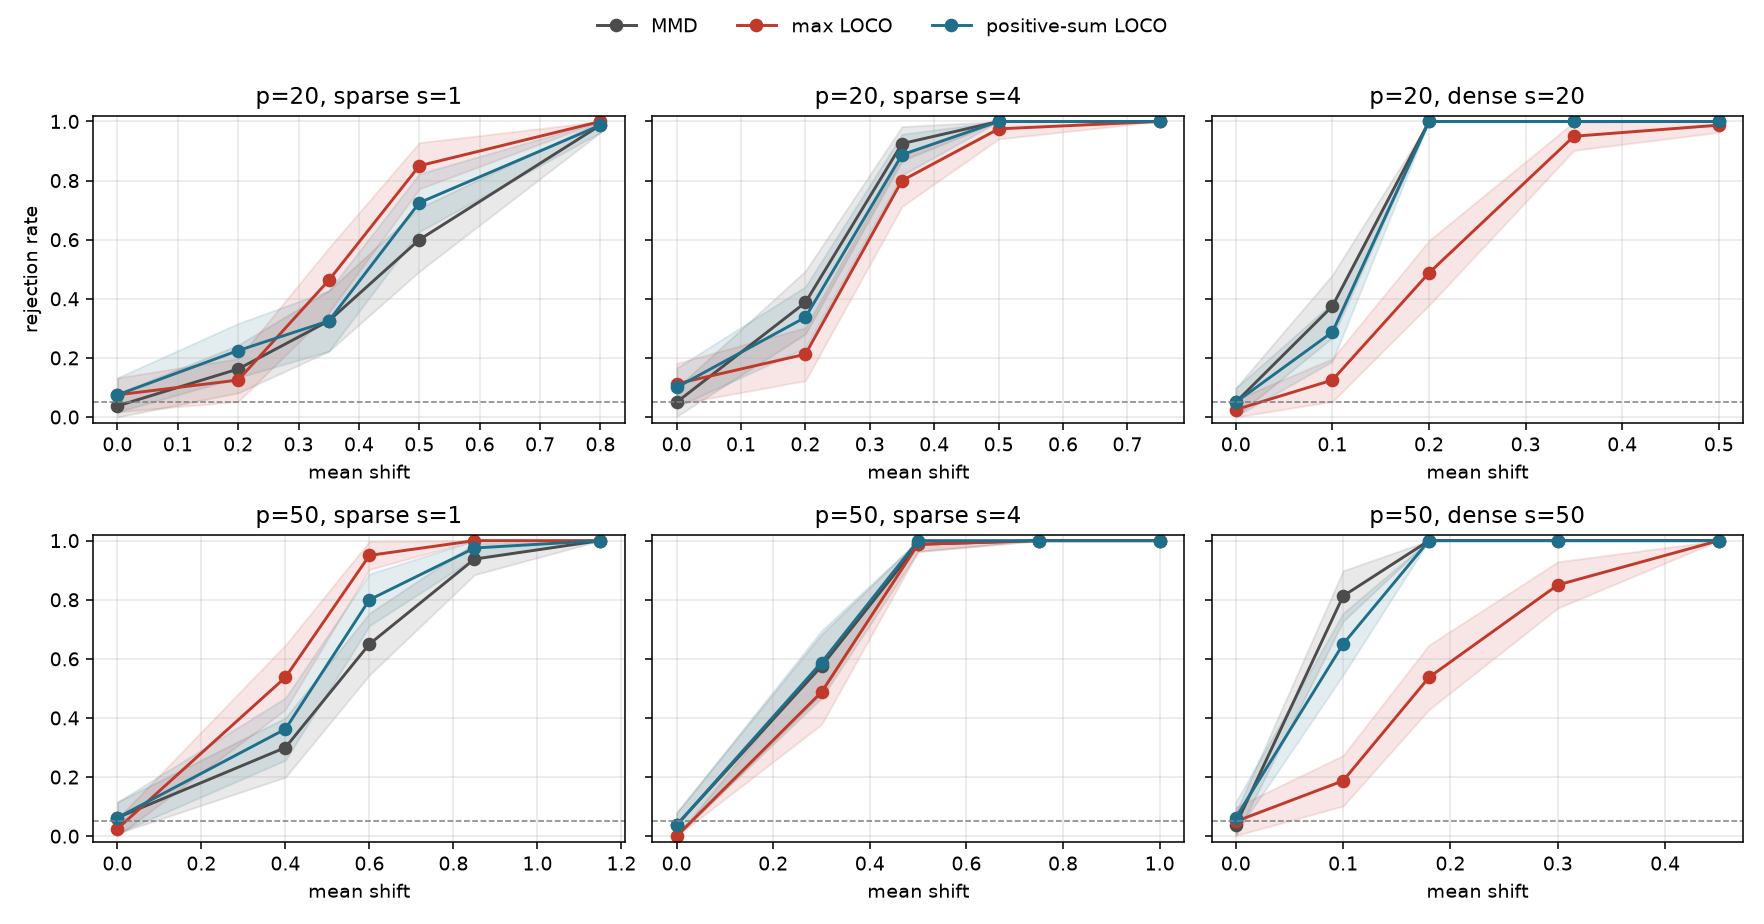
\includegraphics[width=\textwidth]{power.png}
\caption{Independent-coordinate grid. Curves are rejection rates. Bands are
pointwise $1.96$ Monte Carlo standard errors. The horizontal line is $0.05$.}
\end{figure}

\end{document}
